\documentclass[a4paper,12pt]{article}
\usepackage{geometry}
\usepackage{amsmath,amsfonts,amssymb}
\usepackage{graphicx}
\usepackage{subcaption}
\usepackage{caption}
\usepackage{booktabs}
\usepackage{hyperref}
\usepackage{enumitem}
\usepackage{xcolor}
\usepackage{titling}
\usepackage{fancyhdr}
\usepackage{parskip}
\usepackage{listings}
\graphicspath{{outputs/}}

% Custom colors
\definecolor{titleblue}{RGB}{0,102,204}
\definecolor{headingblue}{RGB}{0,51,102}

% Code listing style
\lstset{
    language=Python,
    basicstyle=\ttfamily\small,
    keywordstyle=\color{blue}\bfseries,
    stringstyle=\color{purple},
    commentstyle=\color{gray}\itshape,
    numberstyle=\tiny,
    numbers=left,
    stepnumber=1,
    numbersep=5pt,
    showspaces=false,
    showstringspaces=false,
    frame=single,
    breaklines=true,
    breakatwhitespace=true,
    tabsize=4
}

% Page layout
\geometry{top=2.5cm,bottom=2.5cm,left=2.5cm,right=2.5cm}
\setlength{\parindent}{0pt}
\setlength{\parskip}{1em}

% Header and footer
\pagestyle{fancy}
\fancyhf{}
\fancyhead[L]{\textbf{INS3155 - Computer Vision Midterm Report}}
\fancyhead[R]{\thetitle}
\fancyfoot[C]{\thepage}

% Title customization
\pretitle{\centering\LARGE\bfseries}
\posttitle{\vspace{0.5cm}}

\preauthor{\centering}
\postauthor{}
\predate{\centering}
\postdate{}

\begin{document}

\title{\textcolor{titleblue}{Midterm Project Report}}

\author{\parbox{0.6\linewidth}{\centering
Name: DAO DUC DO\\
Student ID: 23070405\\
Email: 23070405@vnu.edu.vn}}

\date{\today}

\maketitle

\begin{abstract}
This report covers three classic computer vision tasks using traditional (non-deep-learning) methods:
\begin{enumerate}
    \item \textbf{Image Filtering} -- Applying mean, Gaussian, median, and Laplacian filters to reduce noise and sharpen images.
    \item \textbf{3D Reconstruction} -- Using a stereo image pair to estimate depth and build a 3D model.
    \item \textbf{Image Stitching} -- Combining overlapping photos into a single panoramic image.
\end{enumerate}
Each method is evaluated with both visual results and numerical metrics to show what works well and where each approach has limitations.
\end{abstract}

\section{Introduction}

Traditional computer vision methods can solve many image processing problems without needing large datasets or GPU training. This project implements three such methods:

\begin{itemize}
    \item \textbf{Image filtering}: Removing noise from images while trying to keep edges sharp.
    \item \textbf{3D reconstruction}: Estimating depth from two camera views and generating a 3D model.
    \item \textbf{Image stitching}: Joining multiple overlapping photos into one wide panorama.
\end{itemize}

These techniques are widely used in medical imaging, robotics, surveillance, and virtual tours. The report is organized into Part~A (filtering), Part~B (3D reconstruction), and Part~C (stitching).

%% ============================================================
%% PART A
%% ============================================================
\section{Part A: Image Filtering}
\subsection{Methodology}

Four filters were implemented, each with a different approach to handling noise:

\textbf{Mean Filter:} Replaces each pixel with the average of its neighbors using a uniform kernel $h_{mn} = \frac{1}{m \times n}$. Simple and effective, but tends to blur edges.

\textbf{Gaussian Filter:} Similar to the mean filter, but gives more weight to nearby pixels using a bell-curve kernel:
\[
    G(x,y) = \frac{1}{2\pi\sigma^2}e^{-\frac{x^2+y^2}{2\sigma^2}}
\]
This produces smoother results and preserves edges better than the mean filter. We used kernel size $5\times5$ with $\sigma=1.0$.

\textbf{Median Filter:} Replaces each pixel with the \textit{middle value} (median) of its $5\times5$ neighborhood. Particularly good at removing salt-and-pepper noise without blurring.

\textbf{Laplacian Sharpening:} Detects edges using second derivatives and enhances them. Uses the kernel:
$\begin{bmatrix}0&1&0\\1&-4&1\\0&1&0\end{bmatrix}$
Good for making edges stand out, but amplifies noise.

\subsection{Implementation and Results}

\begin{figure}[htbp]
    \centering
    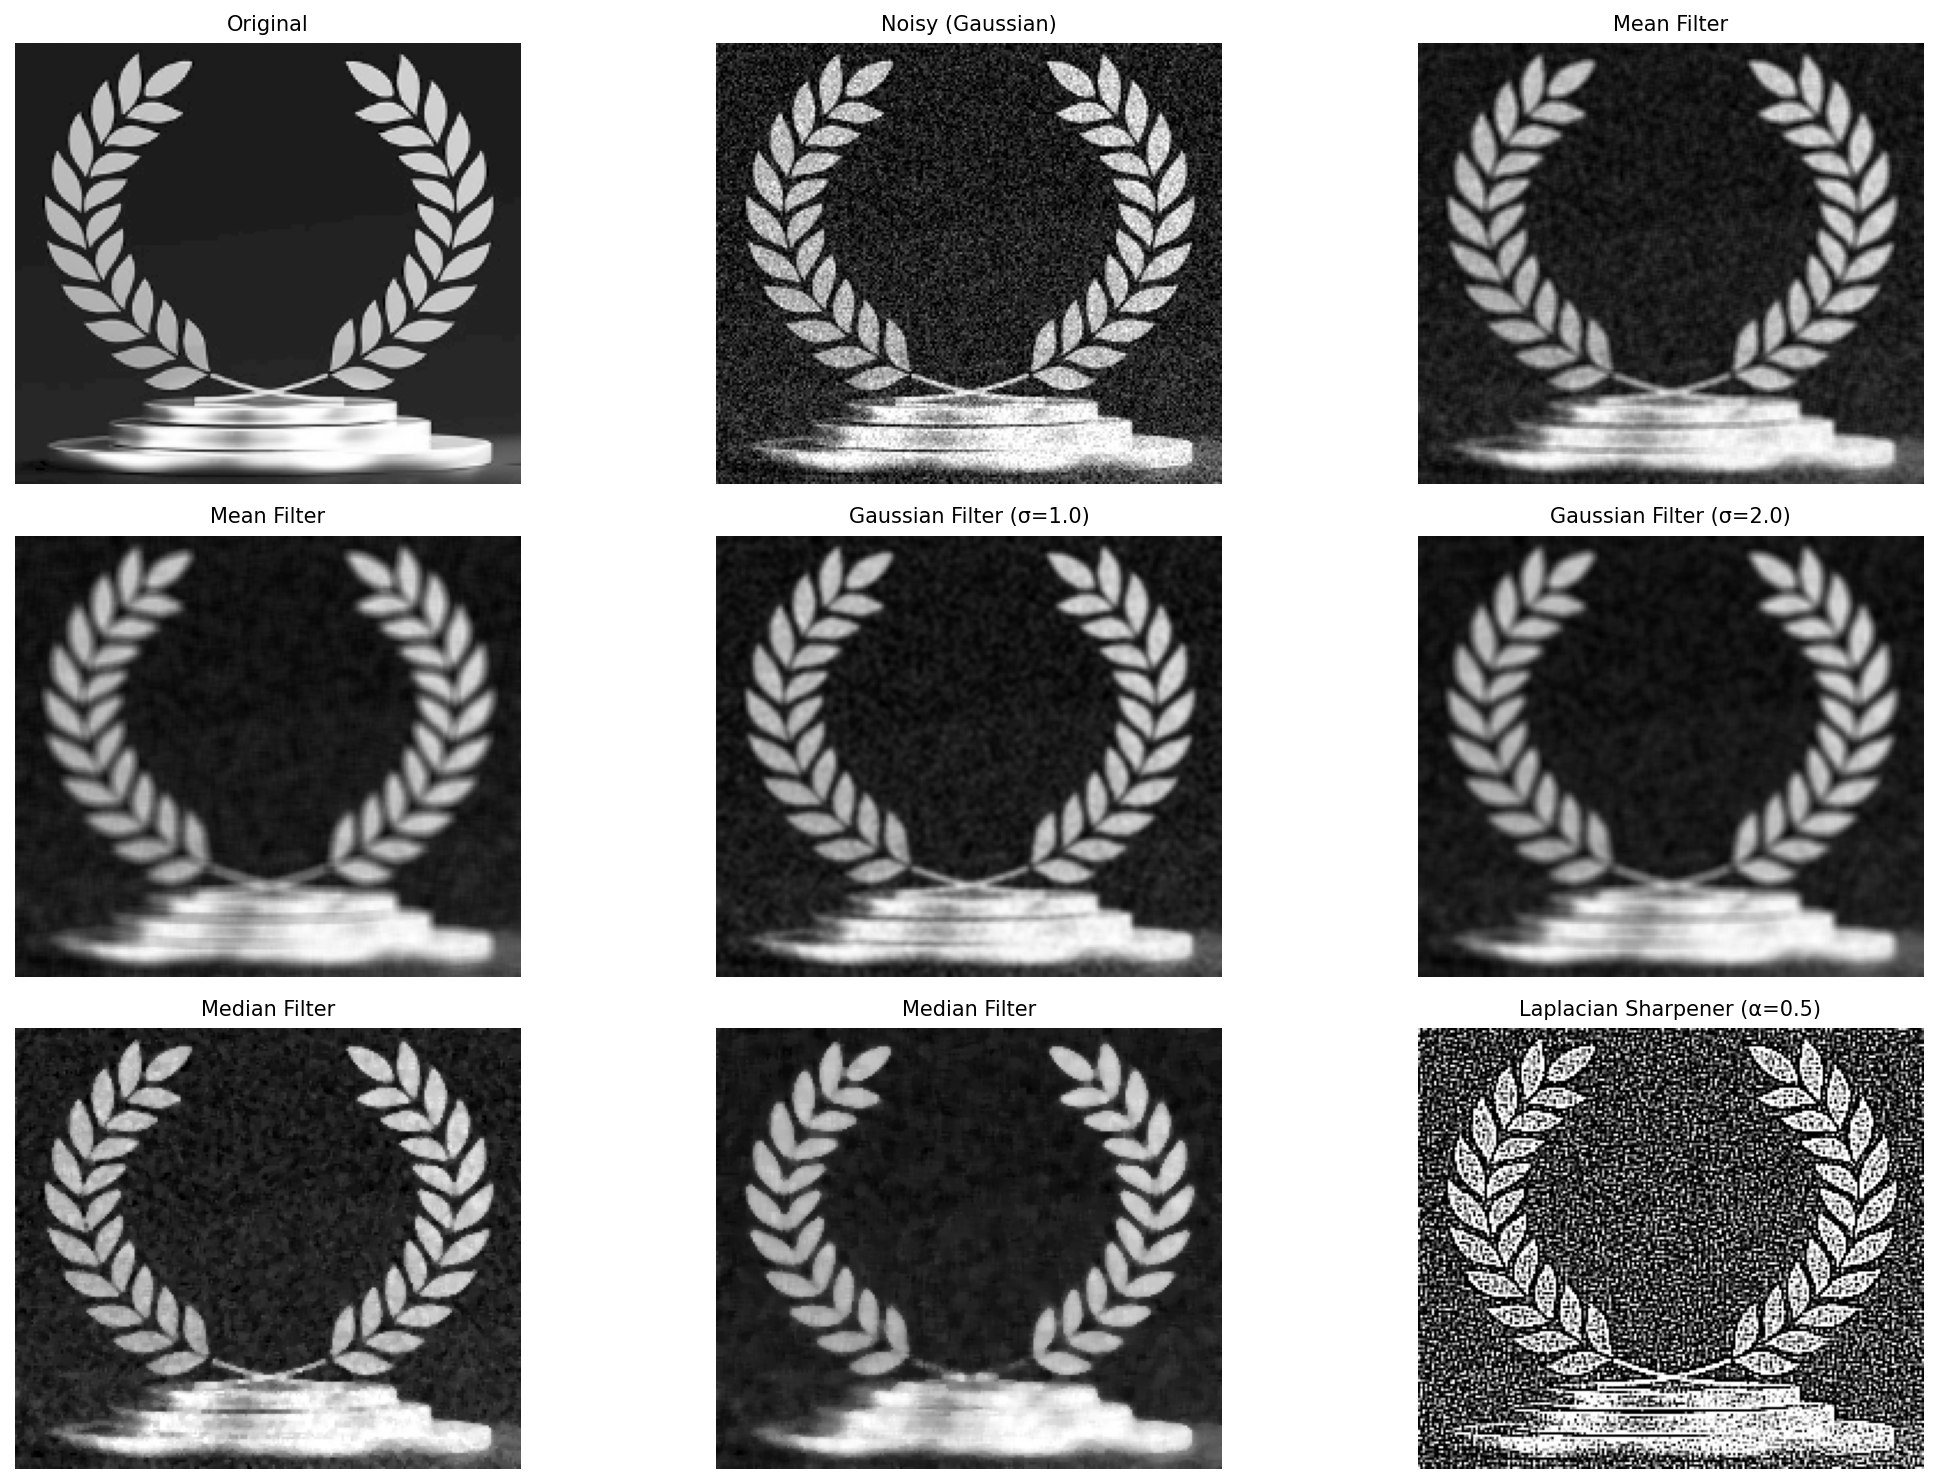
\includegraphics[width=0.9\textwidth]{part_a/filter_comparison.png}
    \caption{Comparison of original, noisy, and filtered images.}
    \label{fig:filter_comparison}
\end{figure}

\subsection{Comparative Analysis}

\subsubsection*{Visual Observations}

\begin{itemize}
    \item \textbf{Mean filter}: Reduces noise well but blurs the image noticeably, especially with larger kernels.
    \item \textbf{Gaussian filter}: Good balance -- smooths noise while keeping edges relatively intact. Increasing $\sigma$ from 1.0 to 2.0 gives more smoothing but also more blur.
    \item \textbf{Median filter}: Best at preserving sharp edges while removing noise. Handles salt-and-pepper noise particularly well.
    \item \textbf{Laplacian sharpener}: Makes edges sharper on clean images, but on noisy images, it makes things \textit{much worse} by amplifying the noise.
\end{itemize}

\begin{figure}[htbp]
    \centering
    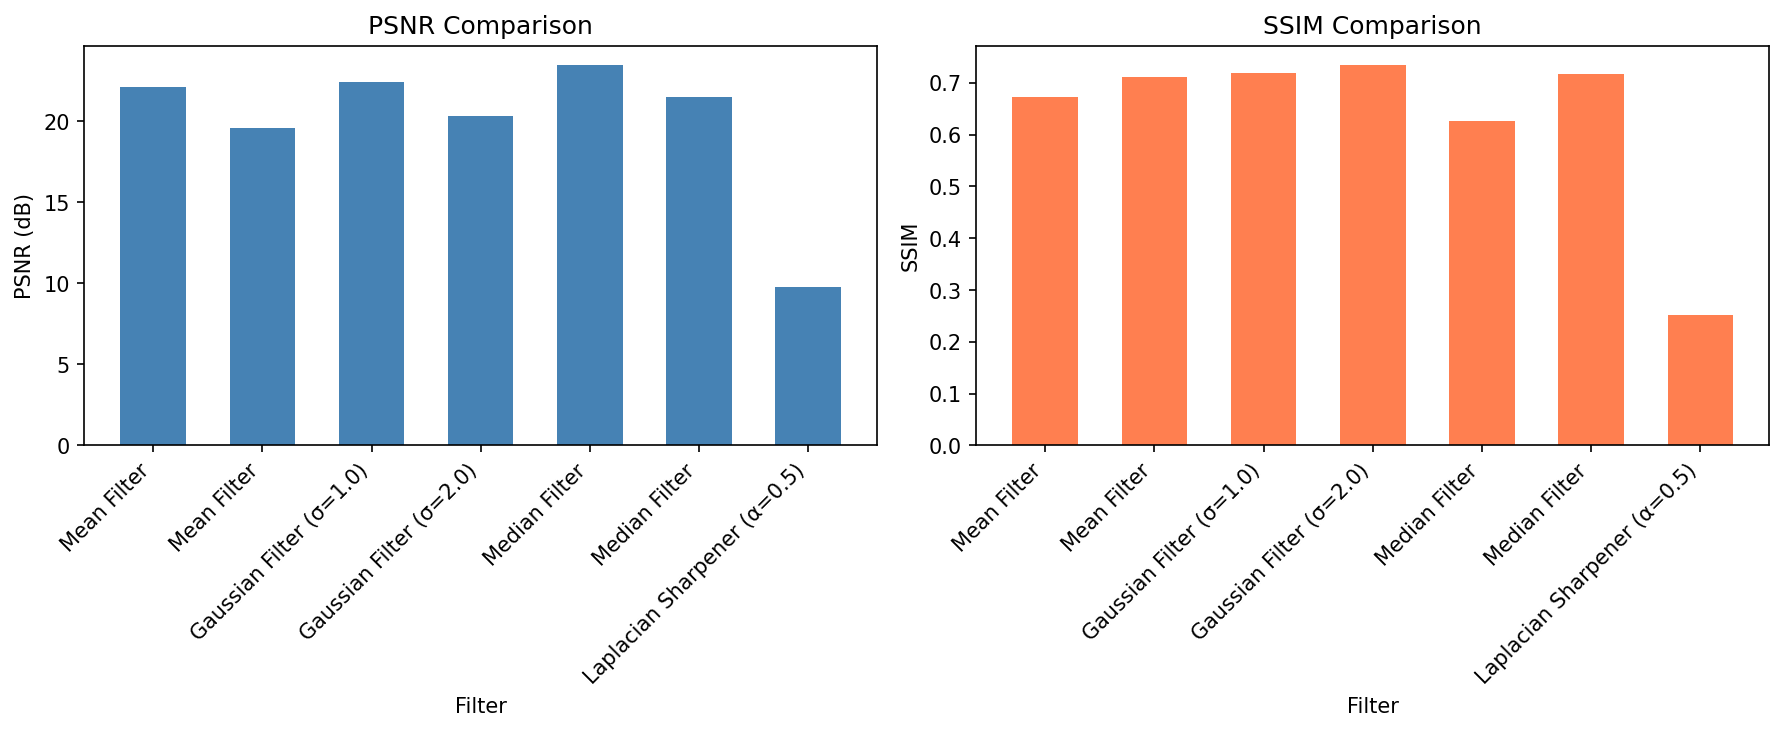
\includegraphics[width=0.9\textwidth]{part_a/metrics_comparison.png}
    \caption{PSNR and SSIM scores for each filter (higher is better).}
    \label{fig:metrics_comparison}
\end{figure}

\subsubsection*{Quantitative Comparison}

We measured two metrics:
\begin{itemize}
    \item \textbf{PSNR} (Peak Signal-to-Noise Ratio): Higher means less pixel-level error.
    \item \textbf{SSIM} (Structural Similarity Index): Higher means the image ``looks'' more like the original to human eyes.
\end{itemize}

\begin{table}[htbp]
    \centering
    \begin{tabular}{|l|c|c|}
        \hline
        \textbf{Filter Type} & \textbf{PSNR (dB)} & \textbf{SSIM} \\ \hline
        Median Filter (Best PSNR) & $\approx 23.5$ & $\approx 0.62$ \\ \hline
        Gaussian Filter ($\sigma=1.0$) & $\approx 22.3$ & $\approx 0.72$ \\ \hline
        Gaussian Filter ($\sigma=2.0$) & $\approx 20.3$ & $\approx 0.73$ \\ \hline
        Laplacian Sharpener ($\alpha=0.5$) & $\approx 9.5$ & $\approx 0.25$ \\ \hline
    \end{tabular}
    \caption{PSNR and SSIM scores for different filters.}
    \label{tab:filter_metrics}
\end{table}

\subsubsection*{Key Takeaways}

\begin{itemize}
    \item \textbf{Median filter} has the highest PSNR ($\approx 23.5$ dB), meaning it removes noise most accurately at the pixel level.
    \item \textbf{Gaussian filter} achieves the highest SSIM ($\approx 0.73$), meaning the filtered image looks most natural to human perception.
    \item Increasing Gaussian $\sigma$ from 1.0 to 2.0 drops PSNR (more blur) but slightly improves SSIM (smoother overall structure).
    \item \textbf{Laplacian sharpener} fails badly on noisy images (PSNR $< 10$ dB), confirming that sharpening should only be applied \textit{after} denoising.
\end{itemize}

\subsubsection*{Summary Table}

\begin{itemize}
    \item \textbf{Median Filter}
    \begin{itemize}
        \item \textit{Best for:} Removing noise while keeping edges sharp.
        \item \textit{Limitation:} May alter textures slightly (lower SSIM).
    \end{itemize}

    \item \textbf{Gaussian Filter ($\sigma=1.0$)}
    \begin{itemize}
        \item \textit{Best for:} Balanced noise reduction with natural-looking results.
        \item \textit{Limitation:} Some residual noise may remain.
    \end{itemize}

    \item \textbf{Gaussian Filter ($\sigma=2.0$)}
    \begin{itemize}
        \item \textit{Best for:} Maximum structural preservation (highest SSIM).
        \item \textit{Limitation:} Over-smoothing blurs fine details.
    \end{itemize}

    \item \textbf{Laplacian Sharpener}
    \begin{itemize}
        \item \textit{Best for:} Edge enhancement on clean, noise-free images.
        \item \textit{Limitation:} Destroys image quality when applied to noisy inputs.
    \end{itemize}
\end{itemize}

%% ============================================================
%% PART B
%% ============================================================
\section{Part B: 3D Reconstruction}
\subsection{Methodology}

The goal is to take two images of the same scene (from slightly different positions) and reconstruct a 3D model. The pipeline has four steps:

\subsubsection*{Step 1: Estimating Depth (Disparity Maps)}

When two cameras view the same object, the object appears at slightly different positions in each image. This difference is called \textbf{disparity}, and it tells us how far away objects are (closer objects have larger disparity).

We implemented two algorithms to compute disparity:

\textbf{Block Matching (BM):} A simple method that compares small blocks of pixels between the left and right images to find the best match:
\[
    d^{*}(x,y) = \arg\min_{d}\;\sum_{(i,j)\in W} \bigl|I_L(x+i,\,y+j) - I_R(x+i-d,\,y+j)\bigr|
\]
Settings: \texttt{numDisparities=64}, \texttt{blockSize=15}.

\textbf{Semi-Global Block Matching (SGBM):} A more advanced method that considers how depth should change smoothly across the image. It checks multiple directions (8 paths) and penalizes sudden depth jumps:
\[
    E(D) = \sum_{p}\left(C(p, D_p) + \sum_{q\in N_p}\left[P_1\cdot\mathbf{1}(|D_p-D_q|=1) + P_2\cdot\mathbf{1}(|D_p-D_q|>1)\right]\right)
\]
Settings: \texttt{numDisparities=64}, \texttt{blockSize=5}.

\subsubsection*{Step 2: Validating Stereo Geometry (Epipolar Lines)}

To verify our stereo pair is correctly set up, we estimate the \textbf{fundamental matrix} $\mathbf{F}$ that describes the geometric relationship between the two views. Using SIFT features and RANSAC, we find $\mathbf{F}$ such that:
\[
    \mathbf{x'}^T \mathbf{F}\, \mathbf{x} = 0
\]
This lets us draw \textbf{epipolar lines} -- if the geometry is correct, matching points in one image should lie on the corresponding epipolar line in the other image.

\subsubsection*{Step 3: Converting Depth to 3D Points}

With disparity $d$ known, we calculate actual depth $Z$ using:
\[
    Z = \frac{f \cdot B}{d}
\]
where $f$ is the focal length and $B$ is the distance between cameras. Each pixel is then projected to 3D:
\[
    X = \frac{(u - c_x) \cdot Z}{f}, \quad Y = \frac{(c_y - v) \cdot Z}{f}
\]

The resulting point cloud is cleaned up using:
\begin{itemize}
    \item Voxel downsampling (merging nearby points)
    \item Outlier removal (removing floating artifacts)
    \item Normal estimation (needed for surface reconstruction)
\end{itemize}

\subsubsection*{Step 4: Building a Surface Mesh}

A triangle mesh is generated from the point cloud using \textbf{Poisson surface reconstruction} (depth=9). The mesh is then cropped to the bounding box of the original point cloud to remove unwanted background.

\subsection{Implementation and Results}

The pipeline was tested on the \textbf{Middlebury Teddy} stereo pair ($450\times375$ pixels).

\textbf{Disparity maps.} Figure~\ref{fig:disparity_comparison} shows the results from both algorithms. BM produces a noisy map with many holes (black areas), especially in smooth regions. SGBM gives a much cleaner and more complete result.

\begin{figure}[htbp]
    \centering
    
\includegraphics[width=0.9\textwidth]{part_b/teddy_clean/comparison.png}
    \caption{Disparity maps: Block Matching (left) vs. SGBM (right).}
    \label{fig:disparity_comparison}
\end{figure}

\textbf{Epipolar geometry.} Figure~\ref{fig:epipolar} confirms the stereo geometry is valid -- matching points lie on their corresponding epipolar lines.

\begin{figure}[htbp]
    \centering
    
\includegraphics[width=0.9\textwidth]{part_b/teddy_clean/epipolar_lines.png}
    \caption{Epipolar lines drawn on both images, confirming valid stereo geometry.}
    \label{fig:epipolar}
\end{figure}

\textbf{3D point cloud.} Using ground truth disparity with camera parameters ($f=500$, $B=0.1$), a colored 3D point cloud was generated (Figure~\ref{fig:pointcloud}).

\begin{figure}[htbp]
    \centering
    
\includegraphics[width=0.9\textwidth]{part_b/teddy_clean/point_cloud_3d.png}
    \caption{3D point cloud from ground truth disparity.}
    \label{fig:pointcloud}
\end{figure}

\textbf{Surface mesh.} Poisson reconstruction produces a smooth surface. Figure~\ref{fig:mesh_render} shows the final mesh.

\begin{figure}[htbp]
    \centering
    
\includegraphics[width=0.9\textwidth]{part_b/teddy_clean/mesh_3d_render.png}
    \caption{3D mesh from Poisson surface reconstruction.}
    \label{fig:mesh_render}
\end{figure}

\subsubsection*{Realistic 3D Renders}

To evaluate the 3D model quality, we rendered it from different angles. Figure~\ref{fig:simu_front} shows the front view (similar to the original camera angle), and Figure~\ref{fig:simu_rotated} shows a rotated view that reveals the depth separation between objects.

\begin{figure}[htbp]
    \centering
    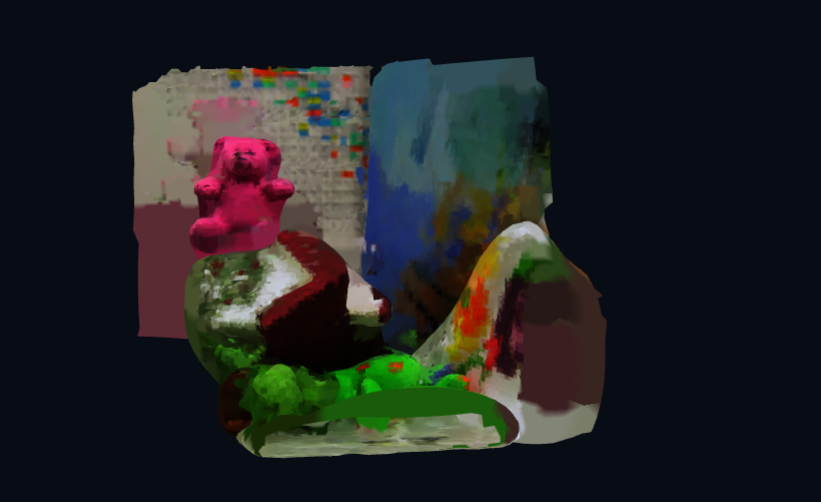
\includegraphics[width=0.85\textwidth]{part_b/teddy_clean/simu.png}
    \caption{3D mesh render -- front view.}
    \label{fig:simu_front}
\end{figure}

\begin{figure}[htbp]
    \centering
    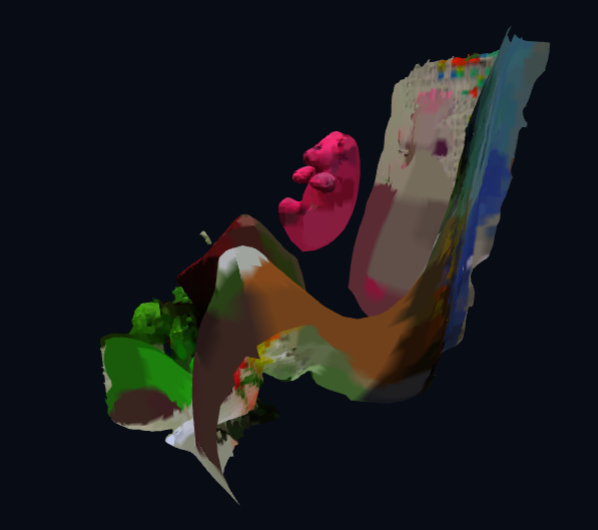
\includegraphics[width=0.85\textwidth]{part_b/teddy_clean/simu2.png}
    \caption{3D mesh render -- rotated view, showing depth layers.}
    \label{fig:simu_rotated}
\end{figure}

\subsection{Comparative Analysis}

\subsubsection*{Block Matching vs.\ SGBM}

\begin{table}[htbp]
    \centering
    \begin{tabular}{|l|c|c|}
        \hline
        \textbf{Criterion} & \textbf{Block Matching} & \textbf{SGBM} \\ \hline
        How it works & Compares local blocks & Optimizes across 8 directions \\ \hline
        Block size & $15\times15$ & $5\times5$ \\ \hline
        Disparity range & 64 & 64 \\ \hline
        Result quality & Noisy, many holes & Smooth, few holes \\ \hline
        Edge preservation & Moderate & Good \\ \hline
        Speed & Fast & Moderate \\ \hline
    \end{tabular}
    \caption{Block Matching vs.\ SGBM comparison.}
    \label{tab:bm_vs_sgbm}
\end{table}

\begin{itemize}
    \item \textbf{Quality:} SGBM clearly wins -- it produces smoother disparity maps with fewer gaps, because it enforces depth smoothness across the whole image.
    \item \textbf{Parameters:} BM needs a large block ($15\times15$) to reduce noise, which hurts edge sharpness. SGBM works well with a small block ($5\times5$) because its smoothness constraints compensate.
    \item \textbf{Speed:} BM is faster since it only does local comparisons. SGBM is better for offline applications where accuracy matters more.
\end{itemize}

\subsubsection*{3D Reconstruction Quality}

The ground truth disparity produces a dense, accurate point cloud. The cleaning steps (voxel downsampling + outlier removal) effectively remove floating artifacts. The Poisson mesh captures the scene surface well, though bounding-box cropping is needed to remove background artifacts.

%% ============================================================
%% PART C
%% ============================================================
\section{Part C: Image Stitching}
\subsection{Methodology}

The goal is to combine multiple overlapping photos into one wide panorama. The pipeline has four stages:

\subsubsection*{Stage 1: Finding Key Points (Feature Detection)}

We need to find distinctive ``landmarks'' in each image that can be recognized across different views.

\textbf{SIFT:} Finds scale-invariant keypoints and creates 128-number descriptors for each. Very accurate but slow.

\textbf{ORB:} A faster alternative using binary descriptors (32 bytes each). About 10$\times$ faster than SIFT, but less distinctive.

\subsubsection*{Stage 2: Matching Key Points}

Descriptors from overlapping images are compared using brute-force matching with KNN ($k=2$). To reject bad matches, we use \textbf{Lowe's Ratio Test}:
\[
    \text{accept match } m \iff \frac{d(m_1)}{d(m_2)} < 0.75
\]
In simple terms: a match is only accepted if the best match is \textit{significantly} closer than the second-best match. This filters out ambiguous matches.

\subsubsection*{Stage 3: Computing the Transformation (Homography)}

From the matched points, we compute a $3\times3$ matrix $\mathbf{H}$ that maps one image onto the other:
\[
    \begin{bmatrix} x' \\ y' \\ 1 \end{bmatrix}
    \sim
    \mathbf{H}
    \begin{bmatrix} x \\ y \\ 1 \end{bmatrix}
\]

RANSAC is used to ignore outlier matches (threshold=4.0, confidence=0.995). At least 4 correct matches are needed.

\subsubsection*{Stage 4: Warping and Blending}

Images are warped onto a common canvas using the homography. In overlapping areas, \textbf{alpha blending} is applied:
\[
    I_{\text{blend}}(x,y) = 0.5 \cdot I_{\text{base}}(x,y) + 0.5 \cdot I_{\text{overlay}}(x,y)
\]
This creates a smooth transition between images. Black borders are automatically cropped from the final result.

\subsection{Implementation and Results}

Both SIFT and ORB were tested on two overlapping landscape images.

\textbf{Feature matching.} Figures~\ref{fig:sift_matches} and~\ref{fig:orb_matches} show the top 50 matches for each detector.

\begin{figure}[htbp]
    \centering
    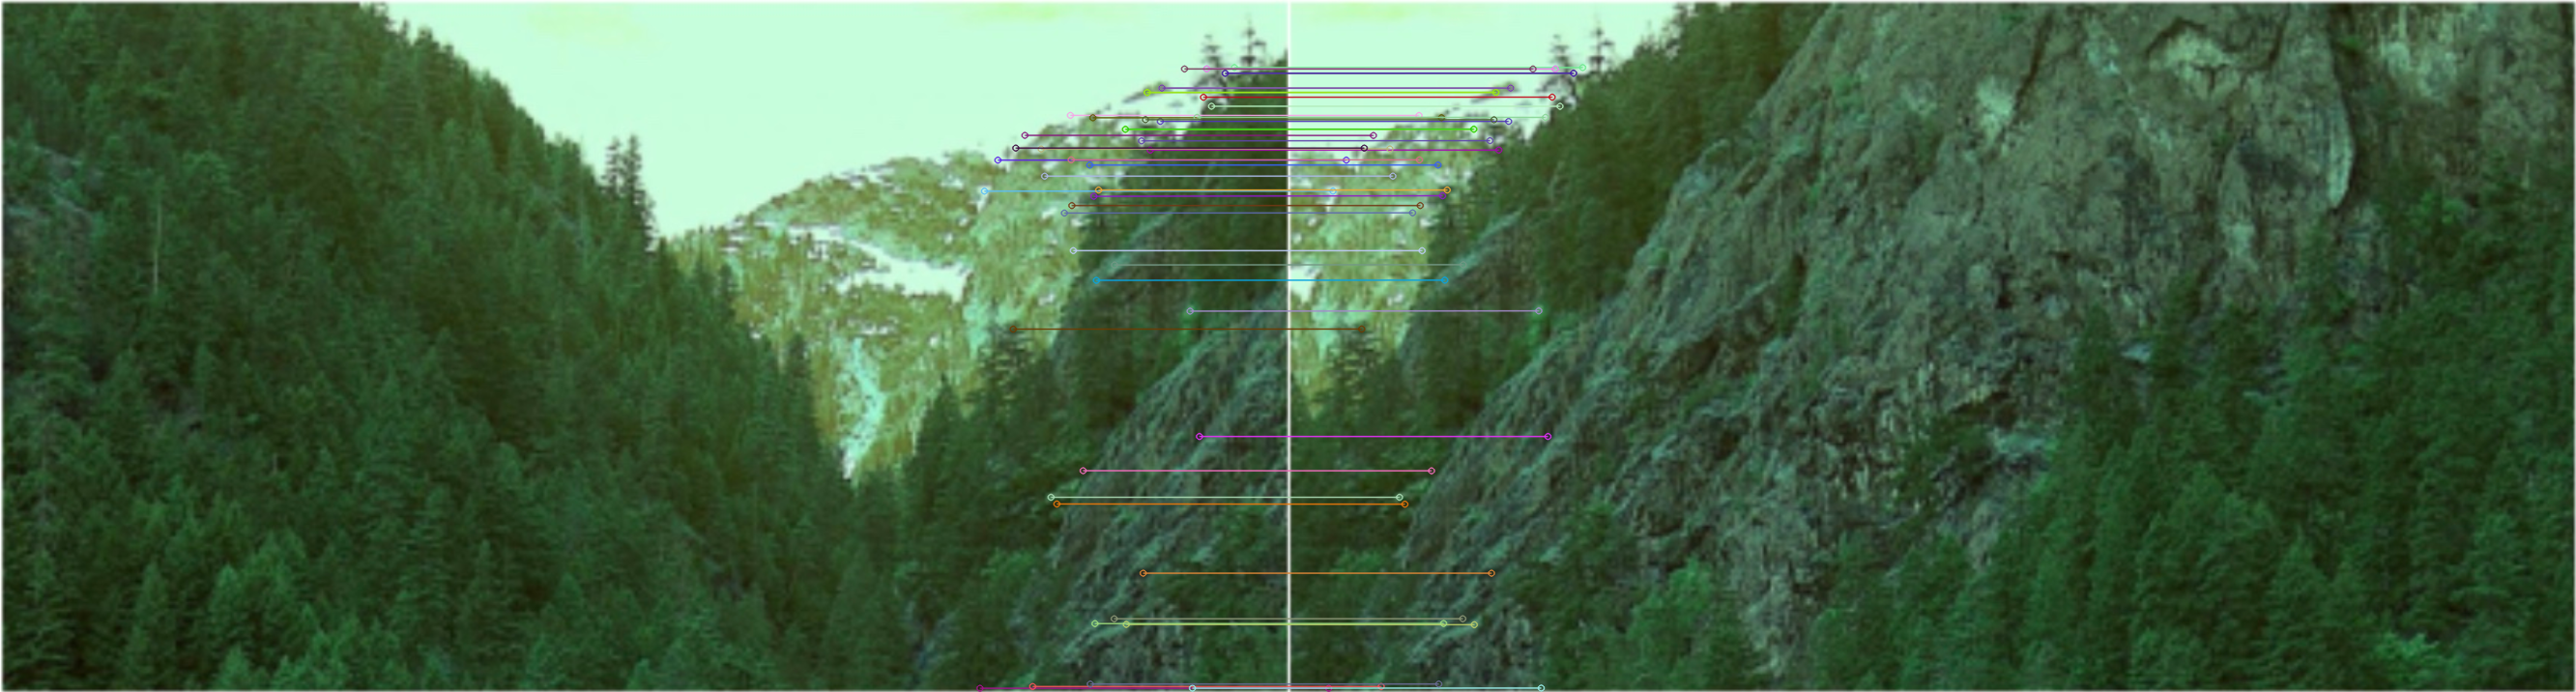
\includegraphics[width=0.9\textwidth]{part_c/matches_sift.png}
    \caption{SIFT feature matches (top 50).}
    \label{fig:sift_matches}
\end{figure}

\begin{figure}[htbp]
    \centering
    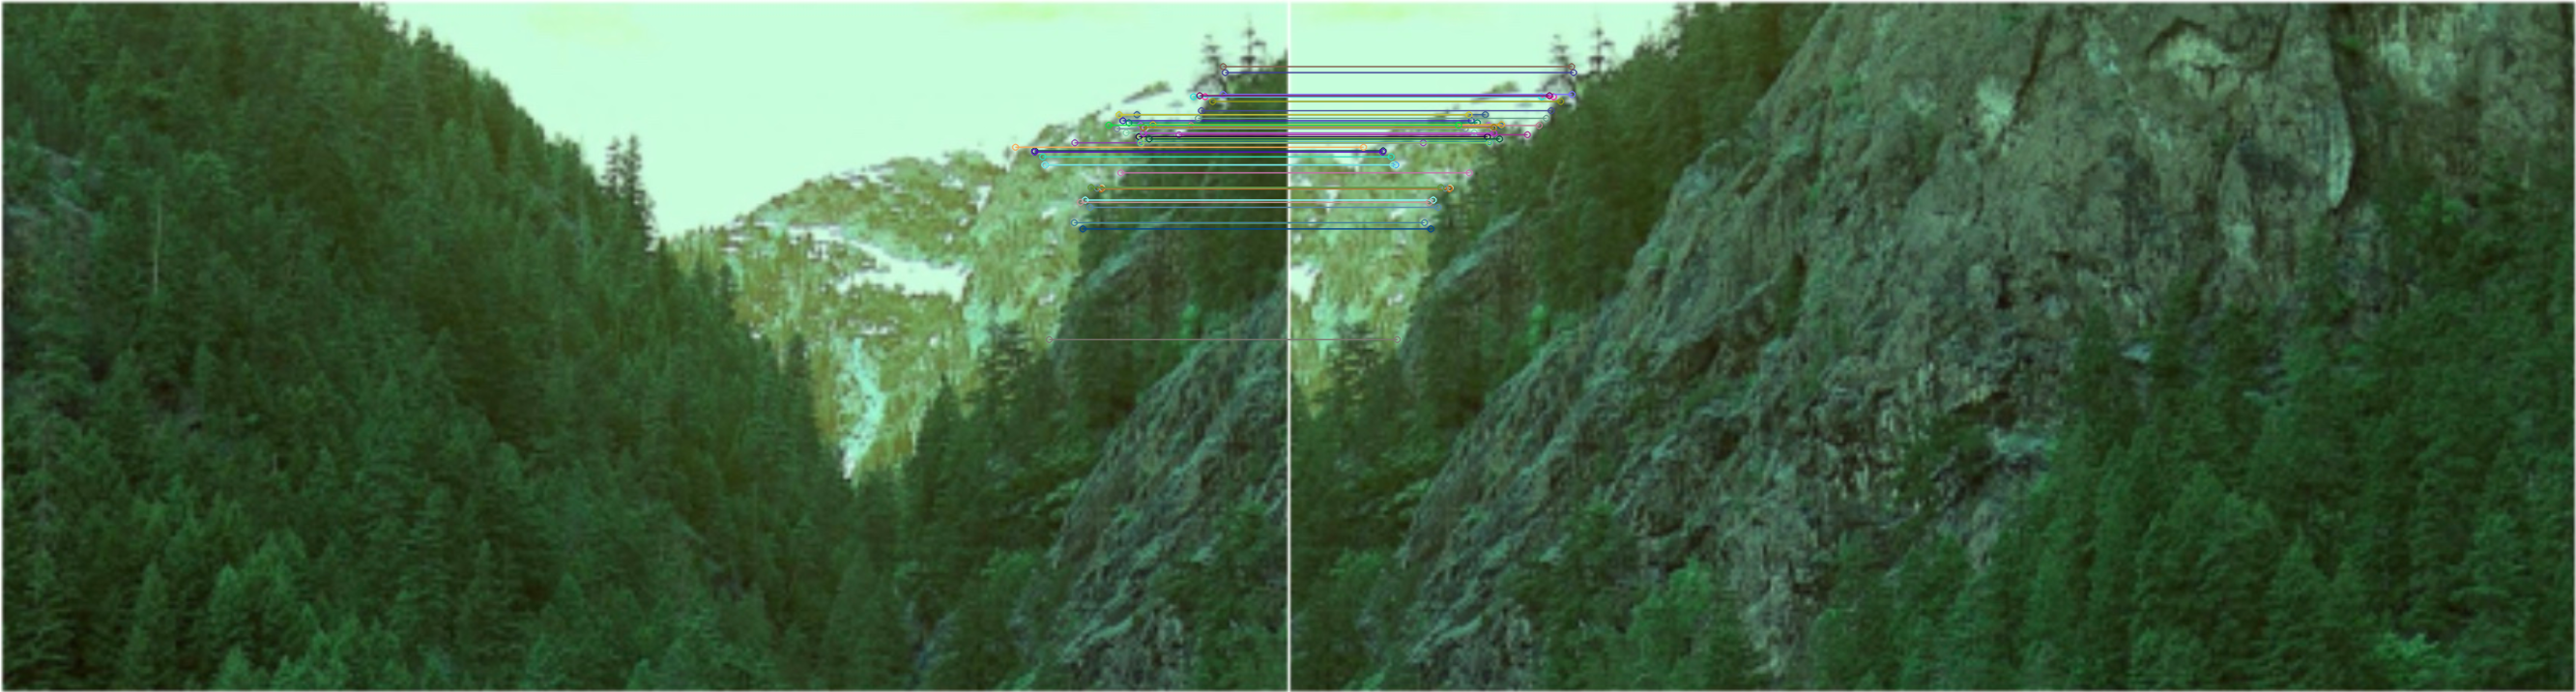
\includegraphics[width=0.9\textwidth]{part_c/matches_orb.png}
    \caption{ORB feature matches (top 50).}
    \label{fig:orb_matches}
\end{figure}

\textbf{Panorama results.} Figures~\ref{fig:panorama_sift} and~\ref{fig:panorama_orb} show the final stitched panoramas.

\begin{figure}[htbp]
    \centering
    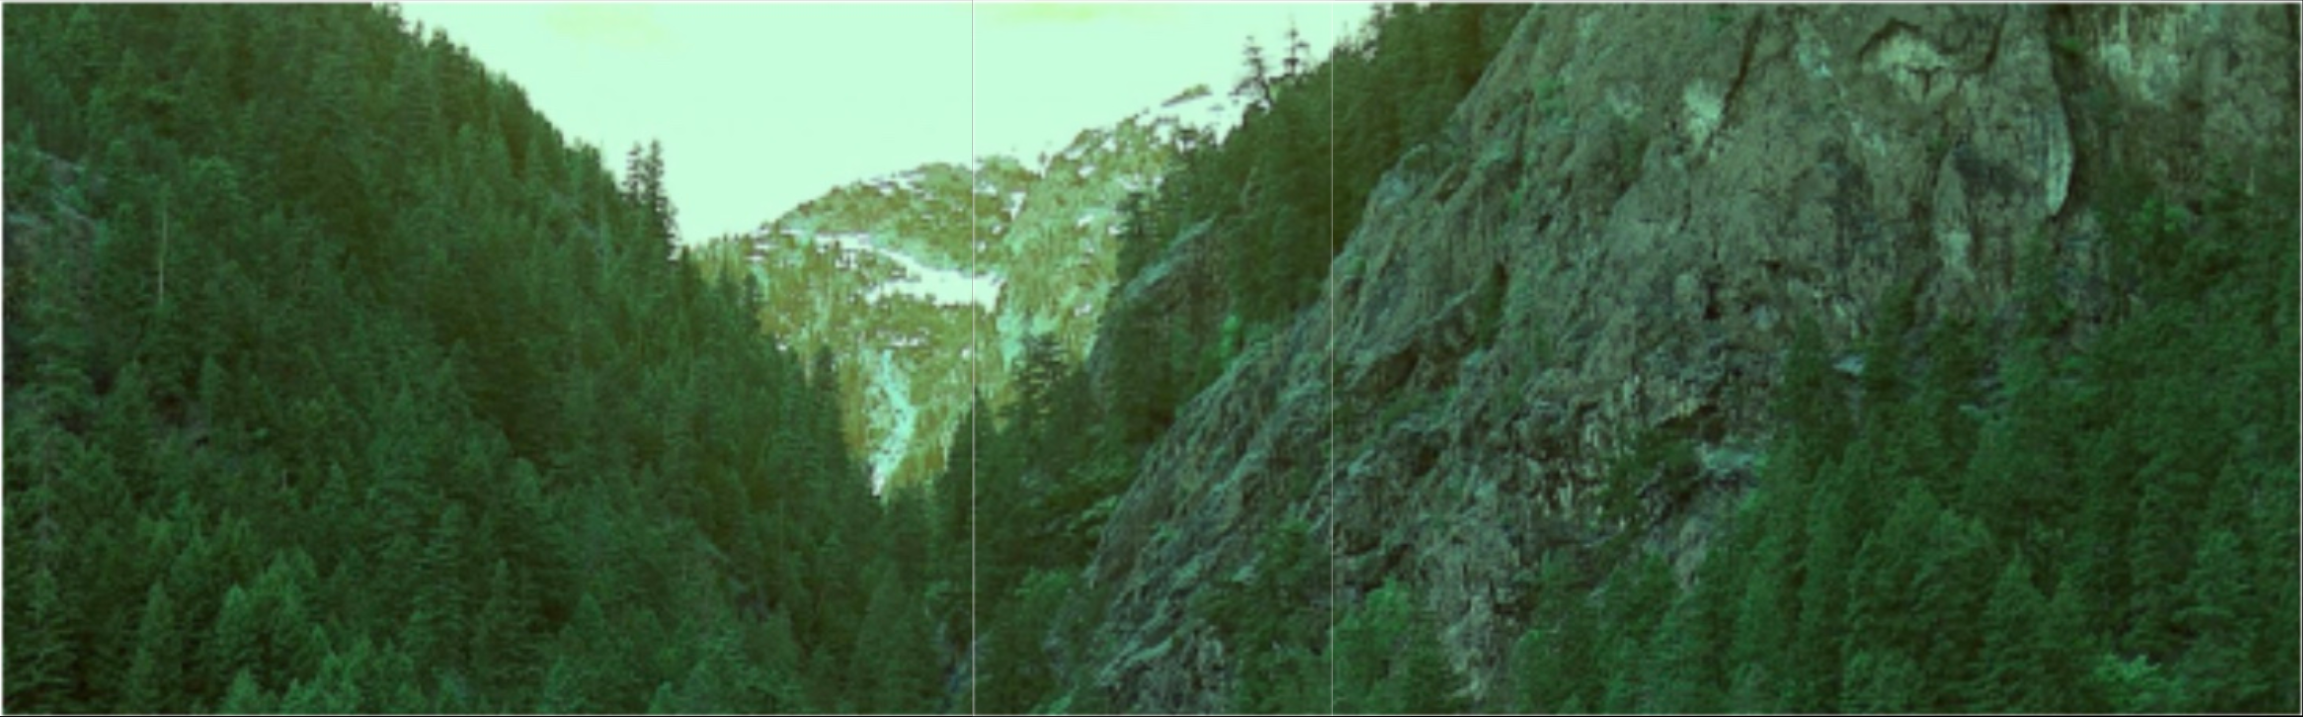
\includegraphics[width=0.9\textwidth]{part_c/panorama_sift.png}
    \caption{Panorama using SIFT.}
    \label{fig:panorama_sift}
\end{figure}

\begin{figure}[htbp]
    \centering
    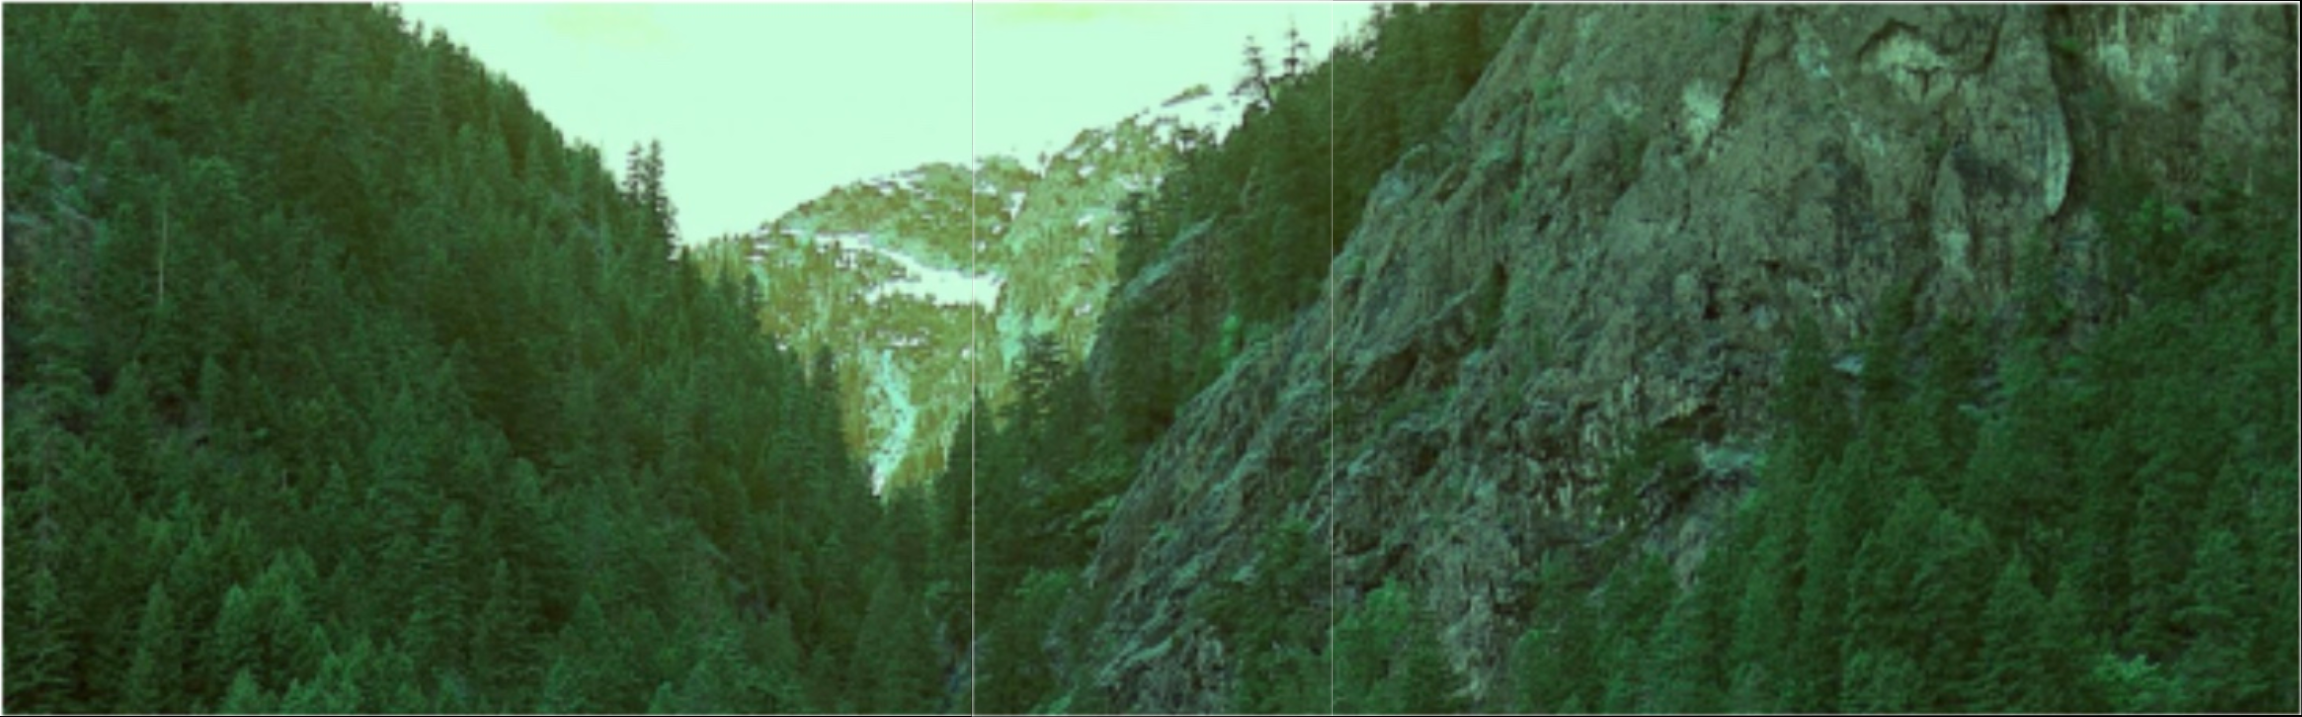
\includegraphics[width=0.9\textwidth]{part_c/panorama_orb.png}
    \caption{Panorama using ORB.}
    \label{fig:panorama_orb}
\end{figure}

\subsection{Comparative Analysis}

\subsubsection*{SIFT vs.\ ORB}

\begin{table}[htbp]
    \centering
    \begin{tabular}{|l|c|c|}
        \hline
        \textbf{Criterion} & \textbf{SIFT} & \textbf{ORB} \\ \hline
        Descriptor size & 128 float numbers & 32 bytes (binary) \\ \hline
        Matching method & L2 distance & Hamming distance \\ \hline
        Scale invariance & Full & Partial \\ \hline
        Rotation invariance & Yes & Yes \\ \hline
        Speed & Slow & Fast ($\sim$10$\times$ faster) \\ \hline
        Max features tested & Unlimited & 2000 \\ \hline
    \end{tabular}
    \caption{SIFT vs.\ ORB feature detectors.}
    \label{tab:sift_vs_orb}
\end{table}

\begin{itemize}
    \item \textbf{Match quality:} SIFT produces more reliable matches because its 128-number descriptors carry richer information, making it easier to distinguish correct from incorrect matches.
    \item \textbf{Panorama quality:} The SIFT panorama (Figure~\ref{fig:panorama_sift}) has better alignment with fewer ghosting artifacts. The ORB panorama may show slight misalignment where wrong matches affected the transformation.
    \item \textbf{Speed:} ORB is $\sim$10$\times$ faster, making it suitable for real-time use (e.g., mobile AR). SIFT is better for offline, high-quality work.
    \item \textbf{Blending:} Both use 50/50 alpha blending, which reduces seams but doesn't fully eliminate color differences. Multi-band blending (e.g., Laplacian pyramid) would improve this further.
\end{itemize}

\subsubsection*{Summary}

\begin{itemize}
    \item \textbf{SIFT}: High accuracy, robust alignment, but slow and originally patented.
    \item \textbf{ORB}: Very fast, open-source, but less accurate due to simpler descriptors.
\end{itemize}

\section{Conclusion}

This project implemented and compared three traditional computer vision pipelines:

\begin{enumerate}
    \item \textbf{Image Filtering}: The \textbf{median filter} is best for removing noise while keeping edges. The \textbf{Gaussian filter} gives the most natural-looking results. The \textbf{Laplacian sharpener} should never be applied directly to noisy images.

    \item \textbf{3D Reconstruction}: \textbf{SGBM} produces much better depth maps than basic Block Matching. Combined with Poisson surface reconstruction, it generates high-quality 3D meshes.

    \item \textbf{Image Stitching}: \textbf{SIFT} gives more accurate panoramas, while \textbf{ORB} is much faster. Both work well for basic stitching tasks.
\end{enumerate}

\textbf{Possible improvements:}
\begin{itemize}
    \item Use multi-band blending (Laplacian pyramid) for smoother panorama transitions.
    \item Combine stereo depth with deep learning (e.g., MiDaS) for better 3D reconstruction.
    \item Automatically select the best filter based on the type of noise detected.
\end{itemize}

\section{References}
\begin{enumerate}
    \item R.~Szeliski, \textit{Computer Vision: Algorithms and Applications}, 2nd ed., Springer, 2022.
    \item G.~Bradski and A.~Kaehler, \textit{Learning OpenCV: Computer Vision with the OpenCV Library}, O'Reilly Media, 2008.
    \item D.~G.~Lowe, ``Distinctive Image Features from Scale-Invariant Keypoints,'' \textit{International Journal of Computer Vision}, vol.~60, no.~2, pp.~91--110, 2004.
    \item E.~Rublee et al., ``ORB: An Efficient Alternative to SIFT or SURF,'' \textit{Proc. IEEE ICCV}, pp.~2564--2571, 2011.
    \item H.~Hirschm{\"u}ller, ``Stereo Processing by Semiglobal Matching and Mutual Information,'' \textit{IEEE Trans. PAMI}, vol.~30, no.~2, pp.~328--341, 2008.
    \item OpenCV Documentation, \url{https://docs.opencv.org/4.x/}.
    \item Open3D Documentation, \url{http://www.open3d.org/docs/release/}.
    \item R.~Ranftl et al., ``Towards Robust Monocular Depth Estimation: Mixing Datasets for Zero-shot Cross-dataset Transfer,'' \textit{IEEE Trans. PAMI}, vol.~44, no.~3, pp.~1623--1637, 2022.
\end{enumerate}

\appendix
\section{Appendix: Python Code}

\subsection{Part A: Image Filtering}

\subsubsection*{Mean Filter (mean\_filter.py)}
\begin{lstlisting}
import cv2
import numpy as np
from src.part_a.filter_interface import ImageFilterInterface

class MeanFilter(ImageFilterInterface):
    """Mean (Box) Filter for image smoothing."""

    def __init__(self, kernel_size: int = 5):
        if kernel_size <= 0 or kernel_size % 2 == 0:
            raise ValueError("Kernel size must be a positive odd integer.")
        self._kernel_size = kernel_size

    @property
    def name(self) -> str:
        return "Mean Filter"

    @property
    def kernel_size(self):
        return (self._kernel_size, self._kernel_size)

    def apply(self, image: np.ndarray) -> np.ndarray:
        return cv2.blur(image, self.kernel_size)
\end{lstlisting}

\subsubsection*{Gaussian Filter (gaussian\_filter.py)}
\begin{lstlisting}
class GaussianFilter(ImageFilterInterface):
    """Gaussian Filter for image smoothing."""

    def __init__(self, kernel_size: int = 5, sigma: float = 1.0):
        if kernel_size <= 0 or kernel_size % 2 == 0:
            raise ValueError("Kernel size must be a positive odd integer.")
        self._kernel_size = kernel_size
        self._sigma = sigma

    @property
    def name(self) -> str:
        return f"Gaussian Filter (sigma={self._sigma})"

    def apply(self, image: np.ndarray) -> np.ndarray:
        return cv2.GaussianBlur(image, self.kernel_size, self._sigma)
\end{lstlisting}

\subsubsection*{Median Filter (median\_filter.py)}
\begin{lstlisting}
class MedianFilter(ImageFilterInterface):
    """Median Filter for noise removal."""

    def __init__(self, kernel_size: int = 5):
        if kernel_size <= 0 or kernel_size % 2 == 0:
            raise ValueError("Kernel size must be a positive odd integer.")
        self._kernel_size = kernel_size

    def apply(self, image: np.ndarray) -> np.ndarray:
        return cv2.medianBlur(image, self._kernel_size)
\end{lstlisting}

\subsubsection*{Laplacian Sharpener (laplacian\_sharpener.py)}
\begin{lstlisting}
class LaplacianSharpener(ImageFilterInterface):
    """Laplacian Sharpening Filter for edge enhancement.
    Formula: sharpened = original - alpha * laplacian(original)
    """

    def __init__(self, kernel_size: int = 3, alpha: float = 1.0):
        valid_sizes = [1, 3, 5, 7]
        if kernel_size not in valid_sizes:
            raise ValueError(f"Kernel size must be one of {valid_sizes}.")
        self._kernel_size = kernel_size
        self._alpha = alpha

    def apply(self, image: np.ndarray) -> np.ndarray:
        laplacian = cv2.Laplacian(image, cv2.CV_64F, ksize=self._kernel_size)
        sharpened = image.astype(np.float64) - self._alpha * laplacian
        return np.clip(sharpened, 0, 255).astype(np.uint8)
\end{lstlisting}

%% ============================================================
\subsection{Part B: 3D Reconstruction}

\subsubsection*{Stereo Matcher -- Block Matching (stereo\_matcher.py)}
\begin{lstlisting}
import cv2
import numpy as np
from src.part_b.stereo_interface import StereoMatcherInterface

class StereoMatcherBM(StereoMatcherInterface):
    """Block Matching stereo algorithm using SAD."""

    def __init__(self, num_disparities=64, block_size=15):
        if num_disparities % 16 != 0:
            raise ValueError("num_disparities must be divisible by 16.")
        self._num_disparities = num_disparities
        self._block_size = block_size
        self._stereo = cv2.StereoBM_create(
            numDisparities=num_disparities, blockSize=block_size)

    def compute_disparity(self, left_image, right_image):
        disparity = self._stereo.compute(left_image, right_image)
        return disparity.astype(np.float32) / 16.0
\end{lstlisting}

\subsubsection*{Stereo Matcher -- SGBM (stereo\_matcher.py)}
\begin{lstlisting}
class StereoMatcherSGBM(StereoMatcherInterface):
    """Semi-Global Block Matching with path-wise cost aggregation."""

    def __init__(self, num_disparities=80, block_size=5,
                 mode=cv2.STEREO_SGBM_MODE_SGBM_3WAY):
        self._num_disparities = num_disparities
        self._block_size = block_size
        p1 = 8 * 3 * block_size ** 2
        p2 = 32 * 3 * block_size ** 2
        self._stereo = cv2.StereoSGBM_create(
            minDisparity=0, numDisparities=num_disparities,
            blockSize=block_size, P1=p1, P2=p2,
            disp12MaxDiff=1, uniquenessRatio=10,
            speckleWindowSize=100, speckleRange=32, mode=mode)

    def compute_disparity(self, left_image, right_image):
        disparity = self._stereo.compute(left_image, right_image)
        return disparity.astype(np.float32) / 16.0
\end{lstlisting}

\subsubsection*{Epipolar Geometry (epipolar\_geometry.py)}
\begin{lstlisting}
class EpipolarGeometry:
    """Computes fundamental matrix and draws epipolar lines."""

    def __init__(self, method=cv2.FM_RANSAC, threshold=3.0):
        self._method = method
        self._threshold = threshold
        self._fundamental_matrix = None

    def compute_fundamental_matrix(self, points_left, points_right):
        """F satisfies: x'.T @ F @ x = 0"""
        pts_l = np.float32(points_left)
        pts_r = np.float32(points_right)
        self._fundamental_matrix, self._inlier_mask = cv2.findFundamentalMat(
            pts_l, pts_r, method=self._method,
            ransacReprojThreshold=self._threshold)
        return self._fundamental_matrix, self._inlier_mask

    def compute_epipolar_lines(self, points, which_image):
        points = np.float32(points).reshape(-1, 1, 2)
        lines = cv2.computeCorrespondEpilines(
            points, which_image, self._fundamental_matrix)
        return lines.reshape(-1, 3)

    @staticmethod
    def draw_epipolar_lines(image, lines, points, colors=None):
        output = cv2.cvtColor(image, cv2.COLOR_GRAY2BGR) \
            if len(image.shape) == 2 else image.copy()
        h, w = output.shape[:2]
        for idx, (line, pt) in enumerate(zip(lines, points)):
            color = colors[idx] if colors else tuple(
                np.random.randint(0, 255, 3).tolist())
            a, b, c = line
            x0, y0 = 0, int(-c / b) if b != 0 else 0
            x1, y1 = w, int(-(c + a * w) / b) if b != 0 else 0
            cv2.line(output, (x0, y0), (x1, y1), color, 1)
            cv2.circle(output, tuple(map(int, pt)), 5, color, -1)
        return output
\end{lstlisting}

\subsubsection*{Point Cloud from Disparity (main.py -- \_create\_3d)}
\begin{lstlisting}
import open3d as o3d

def _create_3d(disparity, color, output_dir):
    """Create point cloud and mesh from ground truth disparity."""
    h, w = disparity.shape
    focal, baseline = 500.0, 0.1
    cx, cy = w / 2, h / 2

    points, colors = [], []
    for v in range(h):
        for u in range(w):
            d = disparity[v, u]
            if d > 10:
                z = (focal * baseline) / (d / 4.0)  # Middlebury scale
                if 0.1 < z < 10:
                    x = (u - cx) * z / focal
                    y = (cy - v) * z / focal
                    points.append([x, y, z])
                    bgr = color[v, u]
                    colors.append([bgr[2], bgr[1], bgr[0]])

    points = np.array(points)
    colors = np.array(colors) / 255.0

    pcd = o3d.geometry.PointCloud()
    pcd.points = o3d.utility.Vector3dVector(points)
    pcd.colors = o3d.utility.Vector3dVector(colors)
    pcd = pcd.voxel_down_sample(voxel_size=0.02)
    pcd, _ = pcd.remove_statistical_outlier(nb_neighbors=30, std_ratio=1.5)
    pcd.estimate_normals()
    pcd.orient_normals_towards_camera_location([0, 0, -5])
    o3d.io.write_point_cloud(f"{output_dir}/pointcloud.ply", pcd)

    # Poisson surface reconstruction
    mesh, _ = o3d.geometry.TriangleMesh.create_from_point_cloud_poisson(
        pcd, depth=9)
    mesh.compute_vertex_normals()
    bbox = pcd.get_axis_aligned_bounding_box()
    mesh = mesh.crop(bbox)
    o3d.io.write_triangle_mesh(f"{output_dir}/mesh.ply", mesh)
    return pcd, mesh
\end{lstlisting}

%% ============================================================
\subsection{Part C: Image Stitching}

\subsubsection*{SIFT Detector (sift\_detector.py)}
\begin{lstlisting}
import cv2
import numpy as np
from src.part_c.detector_interface import FeatureDetectorInterface

class SiftDetector(FeatureDetectorInterface):
    """SIFT-based feature detector."""

    def __init__(self, n_features=0, contrast_threshold=0.04):
        self._detector = cv2.SIFT_create(
            nfeatures=n_features,
            contrastThreshold=contrast_threshold)

    @property
    def norm_type(self):
        return cv2.NORM_L2

    def detect_and_compute(self, image):
        gray = cv2.cvtColor(image, cv2.COLOR_BGR2GRAY) \
            if len(image.shape) == 3 else image
        return self._detector.detectAndCompute(gray, None)
\end{lstlisting}

\subsubsection*{ORB Detector (orb\_detector.py)}
\begin{lstlisting}
class OrbDetector(FeatureDetectorInterface):
    """ORB-based feature detector."""

    def __init__(self, n_features=1000, scale_factor=1.2):
        self._detector = cv2.ORB_create(
            nfeatures=n_features, scaleFactor=scale_factor)

    @property
    def norm_type(self):
        return cv2.NORM_HAMMING

    def detect_and_compute(self, image):
        gray = cv2.cvtColor(image, cv2.COLOR_BGR2GRAY) \
            if len(image.shape) == 3 else image
        return self._detector.detectAndCompute(gray, None)
\end{lstlisting}

\subsubsection*{Feature Matcher (feature\_matcher.py)}
\begin{lstlisting}
class FeatureMatcher:
    """Matches descriptors using BFMatcher with Lowe's ratio test."""

    def __init__(self, norm_type=cv2.NORM_L2, ratio_threshold=0.75):
        self._ratio_threshold = ratio_threshold
        self._matcher = cv2.BFMatcher(norm_type)

    def match(self, descriptors_a, descriptors_b):
        if descriptors_a is None or descriptors_b is None:
            return []
        knn_matches = self._matcher.knnMatch(descriptors_a, descriptors_b, k=2)
        return self._apply_ratio_test(knn_matches)

    def _apply_ratio_test(self, knn_matches):
        good_matches = []
        for match_pair in knn_matches:
            if len(match_pair) < 2:
                continue
            best, second = match_pair
            if best.distance < self._ratio_threshold * second.distance:
                good_matches.append(best)
        return good_matches

    @staticmethod
    def extract_matched_points(kp_a, kp_b, matches):
        src = np.float32([kp_a[m.queryIdx].pt for m in matches]).reshape(-1, 1, 2)
        dst = np.float32([kp_b[m.trainIdx].pt for m in matches]).reshape(-1, 1, 2)
        return src, dst
\end{lstlisting}

\subsubsection*{Homography Estimator (homography\_estimator.py)}
\begin{lstlisting}
class HomographyEstimator:
    """Estimates homography matrix with RANSAC."""

    def __init__(self, ransac_threshold=4.0, confidence=0.995):
        self._ransac_threshold = ransac_threshold
        self._confidence = confidence

    def estimate(self, src_points, dst_points):
        if len(src_points) < 4:
            return None, None, 0
        homography, mask = cv2.findHomography(
            src_points, dst_points, cv2.RANSAC,
            self._ransac_threshold, confidence=self._confidence)
        if homography is None:
            return None, None, 0
        num_inliers = int(mask.sum()) if mask is not None else 0
        return homography, mask, num_inliers
\end{lstlisting}

\subsubsection*{Panorama Builder (panorama\_builder.py)}
\begin{lstlisting}
class PanoramaBuilder:
    """Builds a panorama from multiple overlapping images."""

    def __init__(self, detector, ratio_threshold=0.75, ransac_threshold=4.0):
        self._detector = detector
        self._matcher = FeatureMatcher(
            norm_type=detector.norm_type, ratio_threshold=ratio_threshold)
        self._estimator = HomographyEstimator(ransac_threshold=ransac_threshold)
        self._warper = ImageWarper(blend_mode="alpha")

    def stitch(self, images):
        if len(images) < 2:
            raise ValueError("Need at least 2 images to stitch.")
        result = images[0]
        for i in range(1, len(images)):
            result = self._stitch_pair(result, images[i])
        return self._crop_black_borders(result)

    def _stitch_pair(self, base, next_image):
        kp1, des1 = self._detector.detect_and_compute(base)
        kp2, des2 = self._detector.detect_and_compute(next_image)
        matches = self._matcher.match(des1, des2)
        if len(matches) < 4:
            return base
        src, dst = FeatureMatcher.extract_matched_points(kp1, kp2, matches)
        homography, _, _ = self._estimator.estimate(dst, src)
        if homography is None:
            return base
        canvas_size, offset = self._warper.compute_canvas_size(
            [base, next_image], [np.eye(3), homography])
        base_warped = self._warper.warp_image(base, offset, canvas_size)
        next_warped = self._warper.warp_image(
            next_image, offset @ homography, canvas_size)
        return self._warper.blend_two(base_warped, next_warped)

    @staticmethod
    def _crop_black_borders(image):
        gray = cv2.cvtColor(image, cv2.COLOR_BGR2GRAY)
        _, thresh = cv2.threshold(gray, 1, 255, cv2.THRESH_BINARY)
        contours, _ = cv2.findContours(
            thresh, cv2.RETR_EXTERNAL, cv2.CHAIN_APPROX_SIMPLE)
        if not contours:
            return image
        x, y, w, h = cv2.boundingRect(max(contours, key=cv2.contourArea))
        return image[y:y+h, x:x+w]
\end{lstlisting}

\subsubsection*{Image Warper and Blending (image\_warper.py)}
\begin{lstlisting}
class ImageWarper:
    """Warps images using homography and blends overlapping regions."""

    def __init__(self, blend_mode="alpha"):
        self._blend_mode = blend_mode

    def warp_image(self, image, homography, output_size):
        width, height = output_size
        return cv2.warpPerspective(image, homography, (width, height))

    def blend_two(self, base, overlay):
        base_mask = (base.sum(axis=2) > 0).astype(np.float32)
        overlay_mask = (overlay.sum(axis=2) > 0).astype(np.float32)
        overlap = (base_mask * overlay_mask)[..., np.newaxis]
        if self._blend_mode == "alpha":
            return self._alpha_blend(base, overlay, overlap)
        result = base.copy()
        result[overlay_mask.astype(bool)] = overlay[overlay_mask.astype(bool)]
        return result

    @staticmethod
    def _alpha_blend(base, overlay, overlap_mask):
        base_f = base.astype(np.float32)
        overlay_f = overlay.astype(np.float32)
        blended = np.where(
            overlap_mask > 0,
            base_f * 0.5 + overlay_f * 0.5,
            np.where(overlay_f.sum(axis=2, keepdims=True) > 0,
                     overlay_f, base_f))
        return np.clip(blended, 0, 255).astype(np.uint8)

    def compute_canvas_size(self, images, homographies):
        corners_all = []
        for img, h in zip(images, homographies):
            ih, iw = img.shape[:2]
            corners = np.array(
                [[0,0],[iw,0],[iw,ih],[0,ih]], dtype=np.float32
            ).reshape(-1,1,2)
            corners_all.append(cv2.perspectiveTransform(corners, h))
        all_c = np.concatenate(corners_all, axis=0)
        x_min, y_min = all_c[:,0,0].min(), all_c[:,0,1].min()
        x_max, y_max = all_c[:,0,0].max(), all_c[:,0,1].max()
        offset = np.array([[1,0,-x_min],[0,1,-y_min],[0,0,1]], dtype=np.float64)
        return (int(np.ceil(x_max-x_min)), int(np.ceil(y_max-y_min))), offset
\end{lstlisting}

\end{document}